\documentclass[12pt]{elsarticle}

\usepackage[margin=1.0in]{geometry}
\usepackage{amssymb}
\usepackage{booktabs}
\usepackage{graphicx}
\usepackage{hyperref}
\usepackage{lineno}

\begin{document}

\begin{frontmatter}


\title{Improving Space-Time Image Velocimetry Accuracy with Deep Learning: Integrating Synthetic and Real-World Data}

\author[inst1]{Tenorio, A.}
\author[inst1]{Fernández, R.}
\author[inst2]{Engel, F.}
\author[inst1]{Liu, X.}

\affiliation[inst1]{organization={Pennsylvania State University}, 
			department={Department of Civil and Environmental Engineering},
            city={University Park},
            state={Pennsylvania},
            country={USA}}

\affiliation[inst2]{organization={U.S. Geological Survey}, 
			department={Water Mission Area, Observing Systems Division, Hydrologic Remote Sensing Branch,},
            city={San Antonio},
            state={Texas},
            country={USA}}

\begin{keyword}
STIV \sep Deep Learning \sep Streamflow Measurements \sep Remote Sensing
\end{keyword}

\end{frontmatter}

\linenumbers
\section*{Abstract}
Quantifying streamflow is essential for resource management, habitat monitoring, and emergency response, but extreme events pose challenges for direct measurements due to safety and accessibility concerns. Remote sensing techniques, such as Space-Time Image Velocimetry (STIV), allow for non-contact measurements of velocity and discharge. STIV uses video footage of the water surface to generate Space-Time Images (STI), assuming surface textures will act as passive tracers. However, environmental conditions such as sunlight conditions, surface reflections or rain can hinder the quality of the STIs. While Wavenumber–Frequency Spectra (WFS) filters can improve STI quality, they struggle in real-time applications. Incorporating deep learning can enhance real-time accuracy, as demonstrated in previous work with synthetic STIs. We aim to extend this by combining synthetic, computational, laboratory-controlled, and real-world data to improve the accuracy of flow measurements in natural settings.
\section{Introduction}
Measuring river discharge under natural flow conditions, particularly during floods, remains one of the most challenging tasks in river engineering \cite{fujita2019efficient, fujita2007development, muste2008large}. 

Most recently, STIV started adopting a machine learning approach to improve the accuracy of the velocity estimation. Watanabe et al. proposed a deep learning approach that trains a convolutional neural network (CNN) to estimate the predominant stripe pattern angle of the STI \cite{watanabe2021improving}. The CNN was trained using synthetic STIs with results showing promising performance on STIs from real river footage.

Different approaches have been explored to improve the accuracy and reliability of STIV. \cite{fujita2020application} proposed a method to estimate the velocity of surface waves using a combination of Wavenumber–Frequency Spectra (WFS) filters. The method consist on generating a mask that ignores a portion of the WFS that does not seem to be related to the surface flow. \cite{watanabe2021improving} proposed a deep learning approach that trains a convolutional neural network (CNN) to estimate the predominant stripe pattern angle of the STI. The CNN was trained using synthetic STIs with results showing promising performance on STIs from real river footage.

Relying on CNNs to estimate the stripe pattern angle of the STI is a promising approach, but it is limited by the restraint of a 

Most recently, open-sourced software such as Image Velocimetry Tools (IVy Tools) \cite{engel2025ivytools}


\section{Background}
\subsection{Space-Time Image Velocimetry}
Developed by Fujita et al. \cite{fujita2007development}, the STIV was proposed as an alternative to Large Scale Particle Image Velocimetry (LSPIV) \cite{fujita1998large}. The technique consists of capturing video footage of the water surface and generating a Space-Time Image (STI) from the video frames. The STI is a two-dimensional representation of the water surface, where the x-axis represents space and the y-axis represents time. The x-axis is represented by search lines

with a constant physical length are usually set parallel to the flow direction at regular intervals on the orthorectified image.

The pixel intensity in the STI corresponds to the brightness of the water surface at a given location and time.



...gradient tensor method  further improved in 2018 with a two dimensional autocorrelation function for the image intensity distribution of STI that is used for detecting the most probable texture gradient included in STI \cite{fujita2019efficient}.

\begin{equation}
    R(\tau_x, \tau_y) = \int_{-\infty}^{\infty}\int_{-\infty}^{\infty} f(x, y) f(x - \tau_x, y - \tau_y) dx dy,
\end{equation}

where f(x,y) is the image pixel intensity distribution in the STI and (\(\tau_x, \tau_y\)) are shift space and time parameters.

The mean velocity component at the line segment can be  estimated by
\begin{equation}
    U=\frac{S_x}{S_t}\tan(\theta_{max})
\end{equation}
where $S_x$ is the size of an image pixel and $S_t$ is the time interval between frames. 

Although, STIV remains as a one-dimensional (1D) technique for estimating surface velocities. This assumes the velocity estimates occur along a constant flow direction in the streamwise direction \cite{fujita2019efficient, fujita2020application, fujita2007development,watanabe2021improving}. For an automated technique, this is not ideal since it requires more user intervention, limiting its applicability in real-time or large-scale scenarios. Most recently, Han et al. \cite{han_two-dimensional_2021} proposed  and Legleiter et al. \cite{legleiter2024two} expanded upon a two-dimensional (2D) STIV technique. This approach allows for a more comprehensive analysis of the flow field, enabling the estimation of both velocity and direction without the need for manually inspecting the direction of the flow. However, for a river with lacking obvious water surface features, the 2D-STIV algorithm led to areas of local noise and irregular flow directions \cite{legleiter2024two}.

Building upon the findings of Watanabe et al. \cite{watanabe2021improving} regarding ML-infused STIV and the advancements in 2D-STIV \cite{han_two-dimensional_2021, legleiter2024two}, this paper aims to develop a method that can accurately predict flow velocity and direction from STIs, even under challenging environmental conditions.
\section{Methodology}
\subsection{Data Collection}
The dataset for training the deep learning models was collected in a controlled laboratory environment using the water recirculating flume at the Hydraulics Laboratory, Pennsylvania State University. The flume, measuring XXX m in length, XXX m in width, and XXX m in depth, provided a consistent setting for capturing surface water footage. Videos were recorded under a variety of simulated environmental conditions, including changes in lighting, surface reflections, discharge rates, water depth, presence of obstacles, and artificial rainfall.
\begin{figure}[!htbp]
    \centering
    \begin{minipage}[b]{0.48\textwidth}
        \centering
        \setlength{\fboxsep}{0pt}
        \fbox{\includegraphics[width=\textwidth]{photos/camera_setup.jpg}}
        \textbf{(a)} 
    \end{minipage}
    \hfill
    \begin{minipage}[b]{0.48\textwidth}
        \centering
        \setlength{\fboxsep}{0pt}
        \fbox{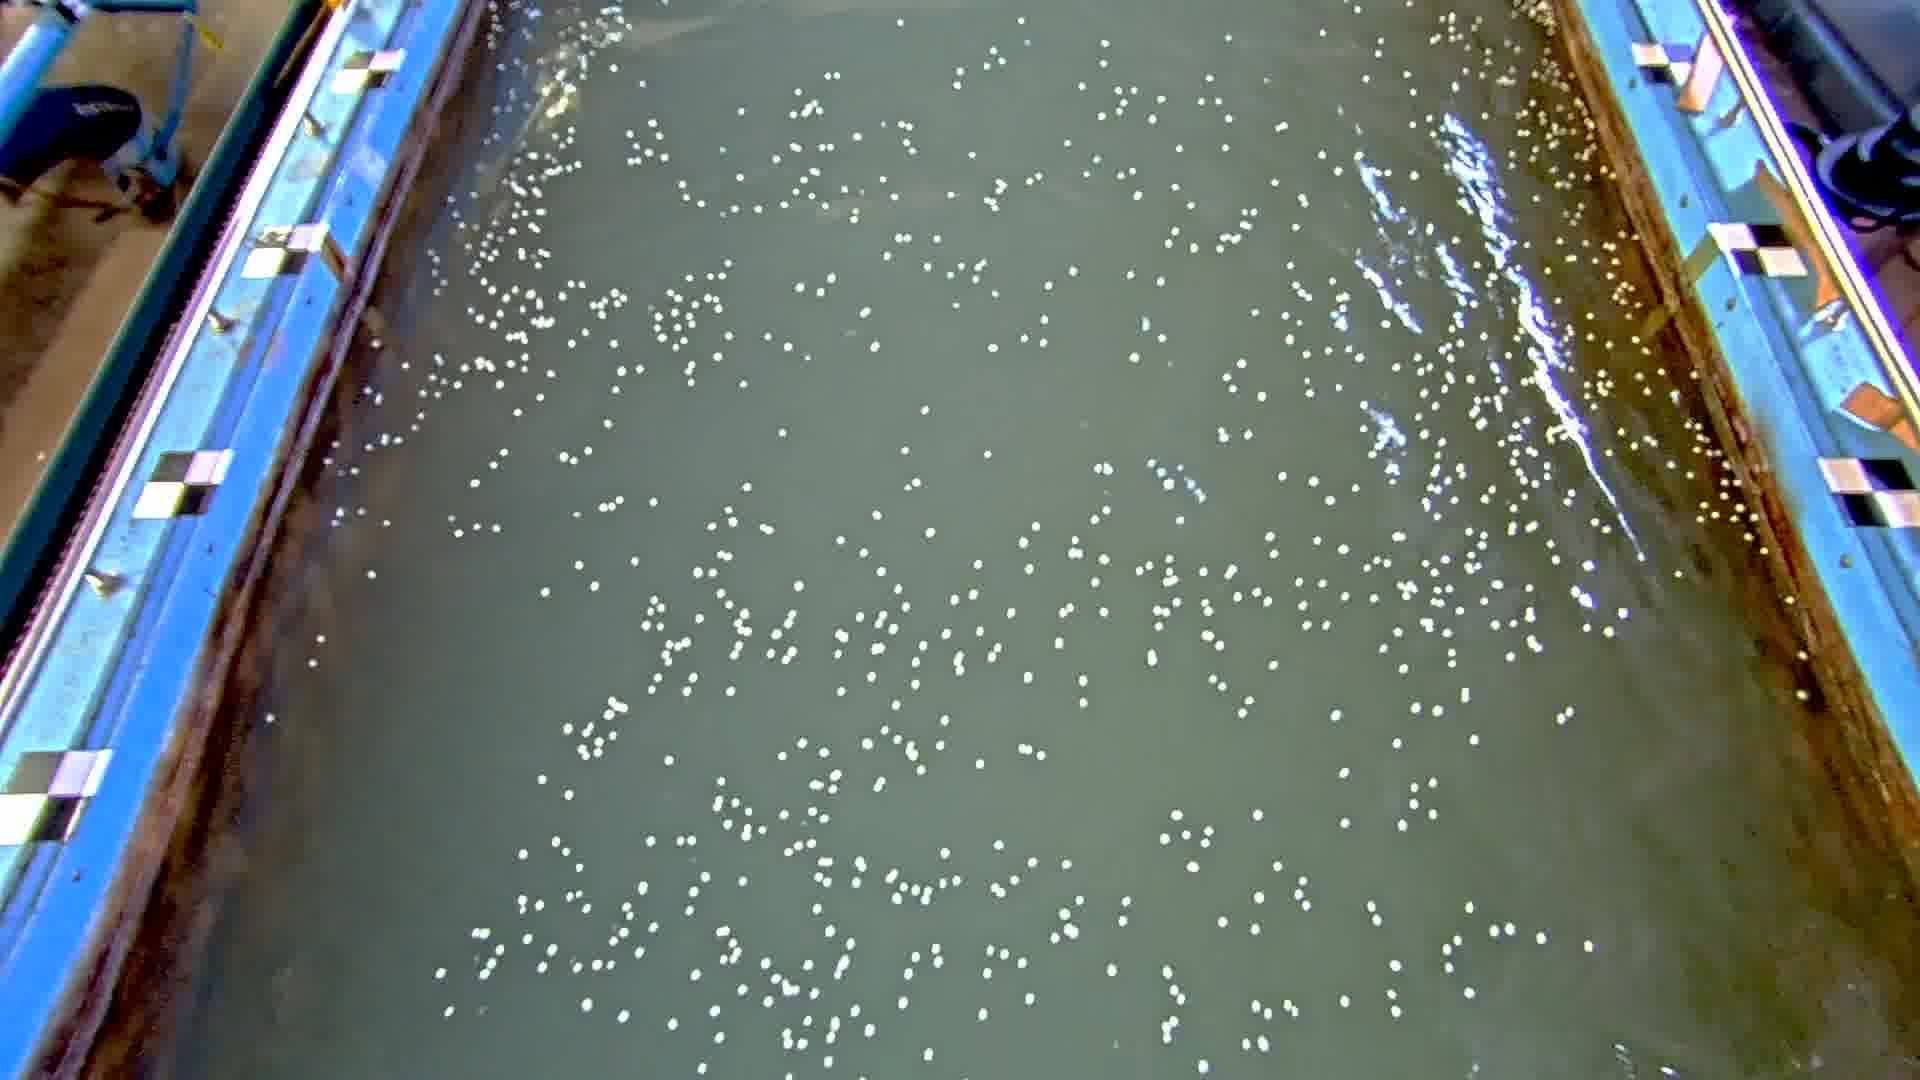
\includegraphics[width=\textwidth]{photos/camera_view.jpg}}
        \textbf{(b)}
    \end{minipage}
    \caption{(a) Experimental camera setup for capturing surface water features in video for STIV. (b) Example camera view including visible seeding particles and designated ground control points (GCPs) every 30 cm.}
    \label{fig:camera_setup}
\end{figure}

Video footage was captured using an AXIS P1385-E network camera mounted on a heavy-duty C-stand (Figure \ref{fig:camera_setup}.a). This camera is designed for outdoor use and provides a resolution of up to 1920×1080 pixels at 60 frames per second (fps). It also features wide dynamic range (WDR) support for challenging lighting conditions, available at up to 30 fps.

A significant requirement of STIV is that there should appear a variation of brightness or color on the water surface moving with the surface flow \cite{fujita2007development}. To ensure this, seeding particles were introduced into the flow to create visible surface patterns that move with the water without interfering with the flow dynamics, Figure \ref{fig:camera_setup}.b. These particles consist of a variety of candle wax beads. The density of the beads is 0.9 g/cm$^3$ with a diameter of XXX mm, which allows them to float on the water surface without sinking. The beads were introduced into the flow ensuring a consistent seeding density across the water surface.
\subsection{Data Preprocessing}
\subsubsection{Space-Time Image Generation}
Video footage was processed to generate Space-Time Images (STIs) using the \textit{IVy Tools} software \cite{engel2025ivytools}. STIs were created using a time window of 128 frames at 60 fps and a spatial resolution of 128 pixels, resulting in images of size 128×128 pixels. The STIs were then converted to grayscale to reduce computational complexity and emphasize texture patterns.

show images of STIs

\subsubsection{Explain the STI stacks generation}

Show STI stacks
\subsection{Deep Learning Architecture}
The angle prediction model employs a Convolutional Neural Network (CNN) architecture. The input to the network is a single-channel 128x128 grayscale STI. The architecture consists of four convolutional blocks and one fully connected (FC) layer, as detailed in Table \ref{tab:cnn_architecture_condensed}. This design allows the network to learn increasingly complex features as it progresses through the layers \cite{zeiler2014visualizing}.

In between convolutions, the specified activation Gaussian Error Linear Unit (GELU) and Batch Normalization layers are applied in sequence. While the Rectified Linear Unit (ReLU) has been a foundational activation function due to its computational efficiency and ability to mitigate vanisihing gradients \cite{pmlr-v15-glorot11a}, recent advancements have shown benefits from smoother activation functions like GELU; helping mitigate the "dying ReLU" problem \cite{hendrycks2016GELU, lu2019dying}. BN is applied to stabilize and accelerate training \cite{ioffe2015batch} by normalizing the outputs of the convolutional layers. Following the convolutional blocks, a Global Average Pooling (GAP) layer is applied to the feature maps to prevent overfitting \cite{lin2013GAP, watanabe2021improving}. 

Here it separates:
\begin{itemize}
    \item \textit{(Predicting flow velocity)} - The output of the GAP layer is then fed into a fully connected (FC) head consisting of two linear layers. Finally, the output is a single value representing the angle of the predominant stripe pattern in the STI. This output is subsequently scaled to the normalized target range of [-0.5, 0.5].
    \item \textit{(Detecting flow direction)}
\end{itemize}


\begin{table}[!htbp]
    \centering
    \caption{CNN Architecture for Angle Prediction from STI Images.}
    \label{tab:cnn_architecture_condensed}
    \resizebox{\columnwidth}{!}{% % Use \columnwidth if in a single column, \textwidth for full page width
    \begin{tabular}{llccccc} 
        \toprule
        Layer Type                & Input Shape         & Output Shape        & Kernel Size & Filters/Units & Activation & Norm. \\
        \midrule
        \multicolumn{6}{l}{\textit{Convolutional Block 1}} \\
        Conv2D                    & 1x128x128           & 32x128x128          & 3x3     & 32            & GELU   & BN2D    \\
        MaxPool2D                 & 32x128x128          & 32x64x64            & 2x2     & ---           & ---  & ---       \\
        \midrule
        \multicolumn{6}{l}{\textit{Convolutional Block 2}} \\
        Conv2D                    & 32x64x64            & 64x64x64            & 3x3     & 64            & GELU   & BN2D    \\
        MaxPool2D                 & 64x64x64            & 64x32x32            & 2x2     & ---           & ---  & ---       \\
        \midrule
        \multicolumn{6}{l}{\textit{Convolutional Block 3}} \\
        Conv2D                    & 64x32x32            & 128x32x32           & 3x3     & 128           & GELU   & BN2D    \\
        MaxPool2D                 & 128x32x32           & 128x16x16           & 2x2     & ---           & ---  & ---       \\
        \midrule
        \multicolumn{6}{l}{\textit{Convolutional Block 4}} \\
        Conv2D                    & 128x16x16           & 128x16x16           & 3x3     & 128           & GELU   & BN2D    \\
        MaxPool2D                 & 128x16x16           & 128x8x8             & 2x2     & ---           & ---  & ---       \\
        GAP  & 128x8x8             & 128x1x1             & 8x8     & 128           & ---   & ---     \\
        Flatten                   & 128x1x1             & 128                 & ---     & ---           & ---  & ---       \\
        \midrule
        \multicolumn{6}{l}{\textit{Fully Connected (FC) Block}} \\
        Linear                    & 128                 & 128                 & ---     & 128           & GELU    & BN1D   \\
        Linear                    & 128                 & 1                   & ---     & 1             & Tanh  & ---      \\
        \bottomrule
    \end{tabular}
    } % End of \resizebox
    \par\medskip\footnotesize
    \textit{Notes:} Both CNNs share the same architecture on the convolutional blocks, but differ in the fully connected (FC) head. The first CNN predicts the angle of the predominant stripe pattern in the STI ($\theta_{max}$), while the second CNN predicts the flow direction ($\phi$). 
\end{table}

\subsection{Detecting flow direction ($\phi$)}


\subsection{Predicting flow velocity ($\theta_{max}$)}
The model is trained using Mean Squared Error (MSE) loss, and the Adam optimizer is employed for optimization. The training process involves minimizing the MSE between the predicted angle and the target angle, which is scaled to the range of [-0.5, 0.5]. The model is trained for 100 epochs with a batch size of 32, using a learning rate of 0.001.

\bibliographystyle{elsarticle-harv}
\newpage
\bibliography{references}

\end{document}